\ProjectEntry
{Analyzing Temperature-Induced Phase Transitions in Pb$_{10-x}$Cu$_x$(PO$_4$)$_6$O}
{Research Independent Study with Prof. Xiawa Wang}
{Phonon/exciton dynamics}
{
  \bitem{Investigated LK-99 thermal behavior (300--500 K) via temperature-dependent XRD, Raman spectroscopy, and DSC.}
  \bitem{Observed reversible structural transitions in XRD (new/shifted peaks) correlating with resistivity jumps.}
  \bitem{Conducted density functional theory (DFT) analysis to interpret observed transitions and spectra.}
  \bitem{Raman modes shift in tandem with resistivity transition; DSC shows no pronounced latent heat.}
  \bitem{Results suggest either minor impurity (e.g., Cu$_2$S) contribution or subtle intrinsic lattice transformation.}
}
{assets/1001_lk99/00_.png}
{\extlink{https://online.flippingbook.com/view/299339187/111/}{MC17 paper} \quad \extlink{https://www.qqgjyx.com/files/p01-LK99-MC17.pdf}{Poster}}
{\badge{Materials Chemistry} \badge{DFT} \badge{MC17}}

\textbf{Technical Highlights:}
We examine temperature-sensitive structural responses in LK-99 that align with electrical resistivity changes. Reversible XRD peak evolution between 300--500 K and concomitant Raman shifts indicate a repeatable transition regime, while DSC lacks strong latent heat signatures.

\begin{figure}[ht]
  \centering
  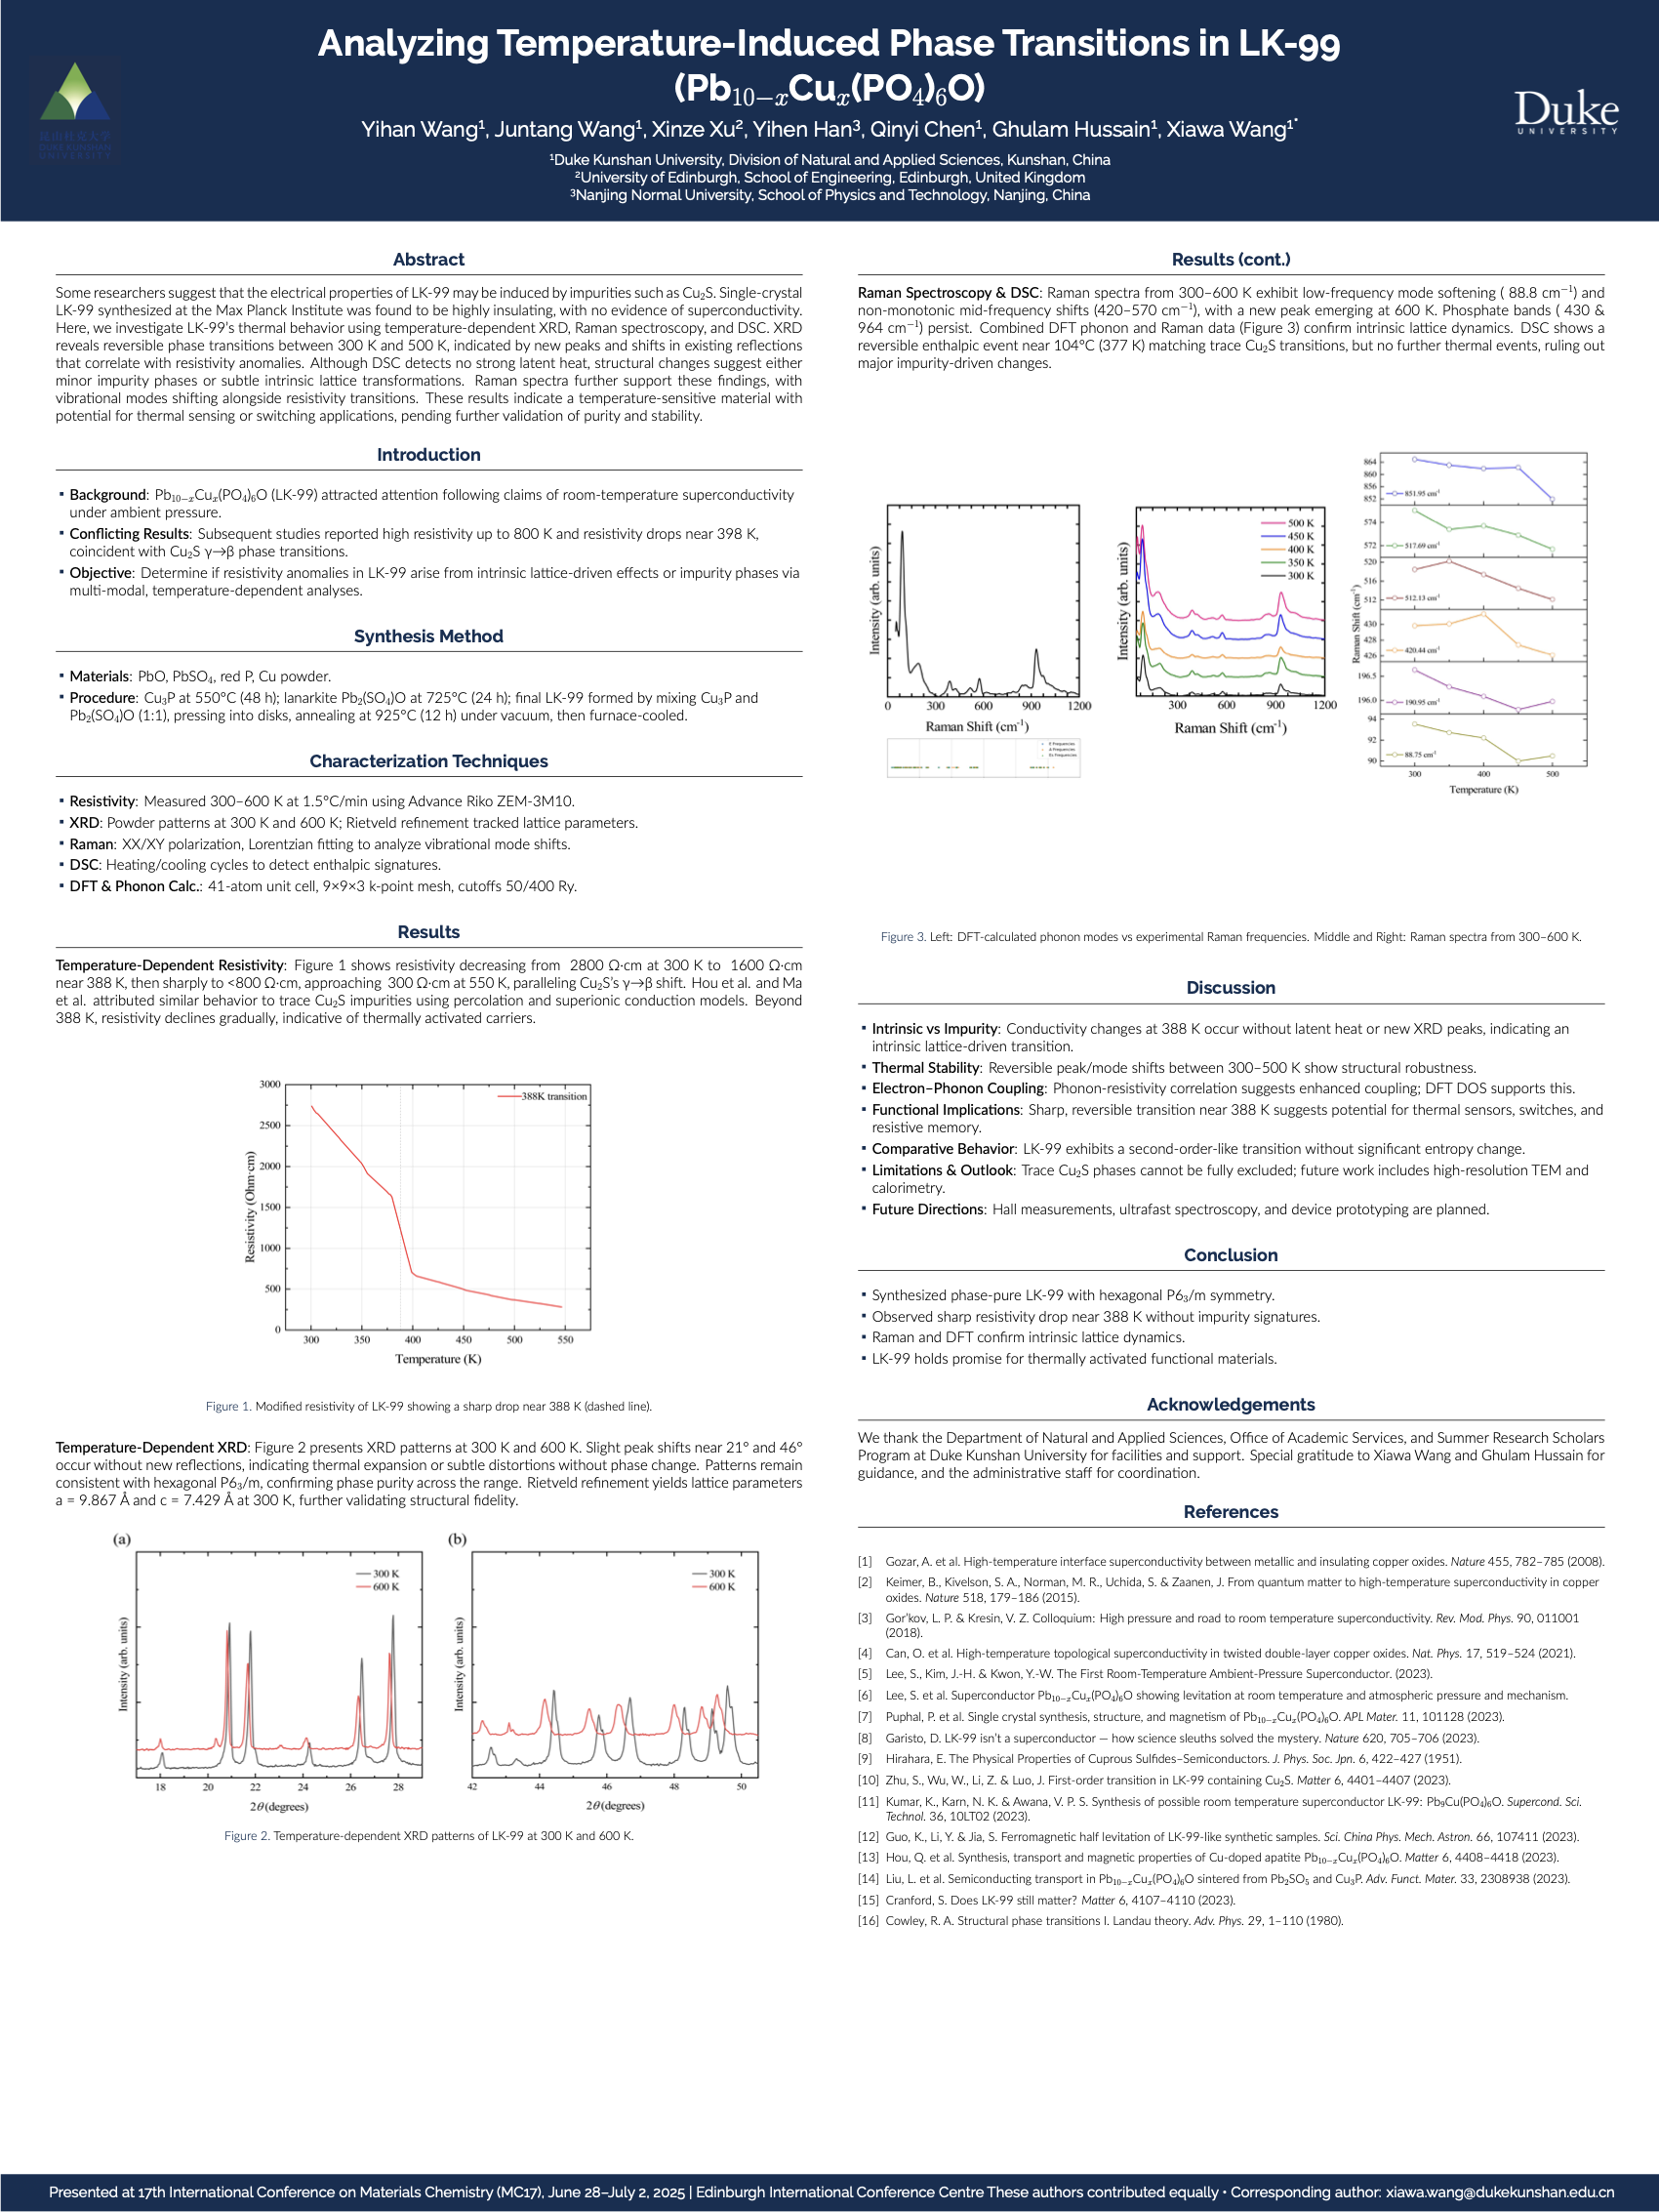
\includegraphics[width=0.8\linewidth]{assets/1001_lk99/00_.png}
  \caption{Temperature-dependent characterization of LK-99. XRD peak evolution and Raman mode shifts track the resistivity transition between 300--500 K; DSC shows no strong latent heat.}
  \label{fig:lk99_temp}
\end{figure}

\textbf{Methodology:}
\begin{itemize}[leftmargin=1.2em, itemsep=0.1em]
  \item Variable-temperature XRD to identify reversible phase/structure evolution
  \item Raman spectroscopy to track vibrational mode shifts across the transition
  \item Differential scanning calorimetry (DSC) to probe latent heat signatures
  \item Resistivity measurements correlated with structural/spectral changes
  \item Density functional theory (DFT) analysis to interpret observed transitions and spectra
\end{itemize}

\textbf{Key Findings:}
\begin{itemize}[leftmargin=1.2em, itemsep=0.1em]
  \item Reversible structural transition correlates with resistivity jumps (300--500 K)
  \item Raman modes shift coherently with structural/electrical changes
  \item Absence of strong DSC peak suggests subtle transformation or low-fraction impurity phase
  \item Thermal/electrical repeatability indicates potential for sensing/switching applications
\end{itemize}

\textbf{Impact:} 
The coupling between structure and electrical response highlights LK-99 as a temperature-sensitive material of interest for functional electronics. Disentangling impurity effects from intrinsic copper-doped lattice behavior requires further microstructural analysis.